% Homework Assignment Article
% LaTeX Template
\documentclass[a4paper,11pt]{article} 

%----------------------------------------------------------------------------------------
%	FORMATTING
%----------------------------------------------------------------------------------------
\usepackage[a4paper, margin=2.5cm]{geometry}
\setlength{\parskip}{0.5em}
\setlength{\parindent}{0in}

%----------------------------------------------------------------------------------------
%	PACKAGES AND OTHER DOCUMENT CONFIGURATIONS
%----------------------------------------------------------------------------------------
\usepackage[utf8]{inputenc} 
\usepackage[T1]{fontenc}
\usepackage{lmodern}
\usepackage[english, spanish]{babel} 
\usepackage{charter} 
\usepackage{microtype} 
\usepackage{amsthm, amsmath, amssymb} 
\usepackage{float} 
\usepackage[final, colorlinks = true, linkcolor = headerBlue, citecolor = headerBlue, urlcolor = headerBlue]{hyperref} 
\usepackage{graphicx, multicol} 
\usepackage{xcolor} 
\usepackage{colortbl} 
\usepackage{array} 
\usepackage{listings} 
\usepackage{booktabs} 

% Configuración de listings
\lstset{
    language=Java,         
    basicstyle=\ttfamily\small,    
    keywordstyle=\color{blue!70!black}\bfseries,
    commentstyle=\color{green!50!black}\itshape,
    numbers=left,            
    frame=lines             
}

% Configuración TikZ
\usepackage{tikz}
\usetikzlibrary{arrows.meta,positioning,fit,backgrounds,calc,shadows} 

\usepackage{fancyhdr} 
\pagestyle{fancy} 
\fancyhead{}\renewcommand{\headrulewidth}{0pt} 
\fancyfoot[L]{} 
\fancyfoot[C]{} 
\fancyfoot[R]{\thepage} 

%----------------------------------------------------------------------------------------
%	UML DIAGRAM CONFIGURATION
%----------------------------------------------------------------------------------------
\definecolor{headerBlue}{HTML}{245C99} 
\definecolor{headerGreen}{HTML}{2D7A4C} 
\definecolor{assocColor}{HTML}{444444} 
\definecolor{inheritColor}{HTML}{222222}

\newcolumntype{L}[1]{>{\raggedright\arraybackslash}p{#1}}

% UML class macro
\newcommand{\umlclass}[7]{%
  \node[inner sep=0pt, outer sep=0pt, drop shadow={opacity=0.25, shadow xshift=2pt, shadow yshift=-2pt}] (#1) at #2 {%
    \scriptsize\sffamily
    \renewcommand{\arraystretch}{1.25}%
    \setlength{\tabcolsep}{6pt}%
    \begin{tabular}{|L{#3}|}
      \hline
      \rowcolor{#4}\multicolumn{1}{|c|}{\textcolor{white}{\bfseries #5}}\\
      \hline
      \rowcolor{white} #6\\
      \hline
      \rowcolor{white} #7\\
      \hline
    \end{tabular}%
  };%
}

\begin{document}

%----------------------------------------------------------------------------------------
%	TITLE SECTION
%----------------------------------------------------------------------------------------

\title{Documentación Técnica: Actividad 3} 
\fancyhead[C]{}
\hrule \medskip 
\begin{minipage}{0.4\textwidth} 
\raggedright
UNAL\\ 
\footnotesize 
\hfill\\
Cristian
\end{minipage}
\begin{minipage}{0.4\textwidth} 
\centering 
\large 
\textbf{Actividad 3}\\ 
\normalsize 
Programación Orientada a Objetos (3007744)\\ 
\end{minipage}
\begin{minipage}{0.18\textwidth} 
\raggedleft
\today\\ 
\footnotesize 
\hfill\\
cristian@unal.edu.co 
\end{minipage}
\medskip\hrule 
\bigskip

%----------------------------------------------------------------------------------------
%	ARTICLE CONTENTS
%----------------------------------------------------------------------------------------

\section{Parte 1: Notas de Estudiantes}
Para esta primera parte armamos una ventana que pide cinco notas. Después de ingresarlas, el programa calcula el promedio, la desviación estándar y nos dice cuál fue la mayor y la menor nota de todas.

\textbf{Cosas extra que le pusimos para que no falle:}
\begin{itemize}
 \item Manejo de errores por si el usuario mete letras en vez de números por accidente.
 \item Nos aseguramos de que no se pueda calcular nada si dejaron algún espacio en blanco.
\end{itemize}

\subsection{Así se ve la interfaz}
Aquí puse unas capturas de cómo funciona el programa paso a paso:

\begin{enumerate}
    \item \textbf{Inicio y Cálculo Correcto:} Primero se abre la ventana vacía esperando las 5 notas. Luego de darle a calcular con buenos datos, muestra los resultados abajo.
    \begin{figure}[htbp]
        \centering
        \begin{minipage}{0.45\textwidth}
            \centering
            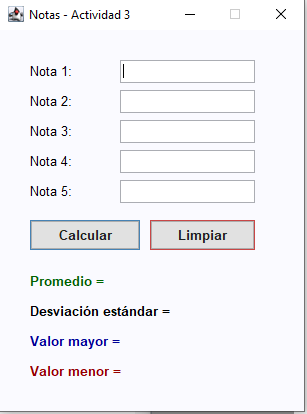
\includegraphics[width=\linewidth]{imagenes/1}
            \caption{Ventana inicial esperando datos.}
        \end{minipage}\hfill
        \begin{minipage}{0.45\textwidth}
            \centering
            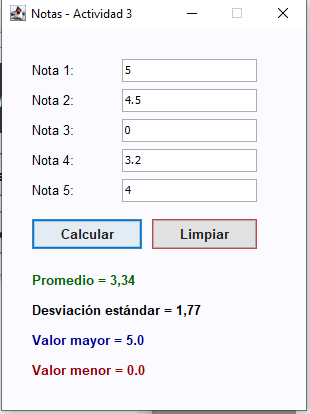
\includegraphics[width=\linewidth]{imagenes/2}
            \caption{Resultados mostrados.}
        \end{minipage}
    \end{figure}

    \item \textbf{Avisos y Errores:} Si falta rellenar algo, sale un aviso. Y si metes texto raro o letras, el programa no se rompe, solo te avisa del error con un cuadro rojo.
    \begin{figure}[htbp]
        \centering
        \begin{minipage}{0.45\textwidth}
            \centering
            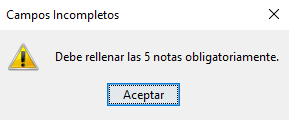
\includegraphics[width=\linewidth]{imagenes/3}
            \caption{Aviso por campos vacíos.}
        \end{minipage}\hfill
        \begin{minipage}{0.45\textwidth}
            \centering
            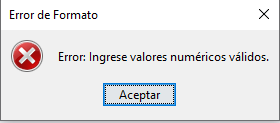
\includegraphics[width=\linewidth]{imagenes/4}
            \caption{Error de formato numérico.}
        \end{minipage}
    \end{figure}
\end{enumerate}

\subsection{Diagrama de Clases (UML)}
Se complementó la información del diagrama para reflejar detalladamente la estructura de la interfaz y la lógica de negocio.

\begin{figure}[htbp] 
\begin{center}
\resizebox{0.85\textwidth}{!}{%
\begin{tikzpicture}[
  font=\sffamily,
  inheritance/.style={draw=inheritColor, line width=1pt, -{Triangle[open, length=8pt, width=10pt]}},
  association/.style={draw=assocColor, line width=0.8pt, -{Latex[length=6pt, width=7pt]}},
  label/.style={font=\scriptsize\sffamily, fill=white, inner sep=2pt, rounded corners=2pt, text=assocColor},
  multiplicity/.style={font=\scriptsize\sffamily, fill=white, inner sep=1pt, text=assocColor}
]

\umlclass{Principal}{(0,0)}{3.0cm}{headerBlue}{Principal}{\strut}{+main(String[] args)\$}

\umlclass{VentanaPrincipal}{(0,-6.5)}{5.5cm}{headerBlue}{VentanaPrincipal}{%
-contenedor: Container\\
-nota1: JLabel\\
-nota2: JLabel\\
-nota3: JLabel\\
-nota4: JLabel\\
-nota5: JLabel\\
-promedio: JLabel\\
-desviacion: JLabel\\
-mayor: JLabel\\
-menor: JLabel\\
-campoNota1: JTextField\\
-campoNota2: JTextField\\
-campoNota3: JTextField\\
-campoNota4: JTextField\\
-campoNota5: JTextField\\
-calcular: JButton\\
-limpiar: JButton}{%
+VentanaPrincipal()\\
-inicio()\\
+actionPerformed(ActionEvent evento)}

\umlclass{Notas}{(0,-15.5)}{4.8cm}{headerGreen}{Notas}{%
\textasciitilde{}listaNotas: double[]}{%
+Notas()\\
\textasciitilde{}calcularPromedio(): double\\
\textasciitilde{}calcularDesviacion(): double\\
\textasciitilde{}calcularMenor(): double\\
\textasciitilde{}calcularMayor(): double}

\begin{scope}[on background layer]
  \node[
    draw=headerBlue!50,
    dashed,
    rounded corners=8pt,
    very thick,
    fill=headerBlue!5,
    inner xsep=25pt,
    inner ysep=25pt,
    fit=(Principal) (VentanaPrincipal) (Notas)
  ] (namespace) {};
  \node[
    anchor=south west,
    text=headerBlue,
    font=\bfseries\sffamily
  ] at (namespace.north west) {Paquete: Notas};
\end{scope}

\draw[association] (Principal.south) -- (VentanaPrincipal.north)
  node[label, midway, right] {Inicia ventana}
  node[multiplicity, near start, left] {1}
  node[multiplicity, near end, left] {1};

\draw[association] (VentanaPrincipal.south) -- (Notas.north)
  node[label, midway, right] {Instancia para cálculos}
  node[multiplicity, near start, left] {1}
  node[multiplicity, near end, left] {1};

\end{tikzpicture}
}
\end{center}
\end{figure}

\subsection{Cómo funciona por detrás}
\begin{itemize}
    \item \textbf{Cálculo:} Cuando metes las notas y le das a calcular, el código lee los textos, los convierte a números y llama a la clase Notas para hacer las matemáticas.
    \item \textbf{Reinicio:} Con el botón Limpiar se borran todos los campos de texto para poder hacer otro cálculo rápido.
    \item \textbf{Protección:} Le pusimos un bloque \textit{try-catch} para atrapar los \textit{NumberFormatException} y evitar que la app se caiga.
\end{itemize}


\section{Parte 2: Cálculo de Figuras Geométricas}
En esta segunda parte hicimos un programa para sacar el volumen y la superficie de tres figuras tridimensionales: Cilindro, Esfera y Pirámide. Utilizamos herencia, donde todas las figuras concretas heredan sus datos principales de una superclase genérica.

\subsection{Vistas de la aplicación}
La aplicación está dividida por pequeñas ventanas para cada figura.

\begin{enumerate}
    \item \textbf{Menú principal de figuras:} Al principio sale este menú para escoger qué figura quieres calcular.
    \begin{figure}[htbp]
        \centering
        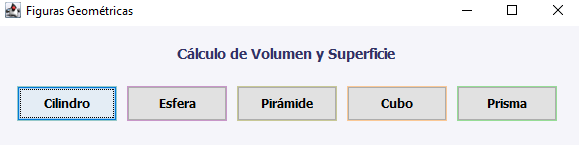
\includegraphics[width=0.45\textwidth]{imagenes/5}
        \caption{Ventana inicial de selección.}
    \end{figure}

    \item \textbf{Ventanas de cada figura:} Al abrirse, cada una pide los datos que necesita específicamente para su fórmula.
    \begin{figure}[htbp]
        \centering
        \begin{minipage}{0.31\textwidth}
            \centering
            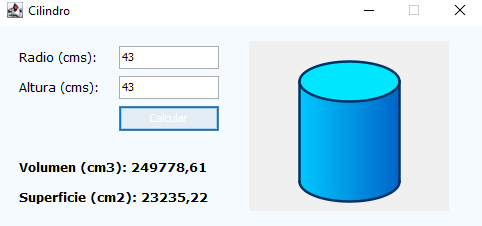
\includegraphics[width=\linewidth]{imagenes/6}
            \caption{Datos del Cilindro.}
        \end{minipage}\hfill
        \begin{minipage}{0.31\textwidth}
            \centering
            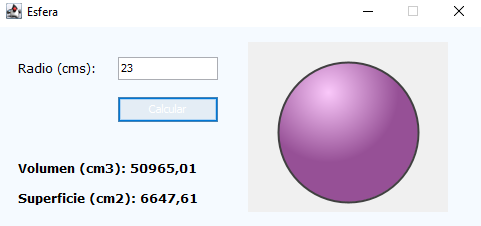
\includegraphics[width=\linewidth]{imagenes/7}
            \caption{Datos de la Esfera.}
        \end{minipage}\hfill
        \begin{minipage}{0.31\textwidth}
            \centering
            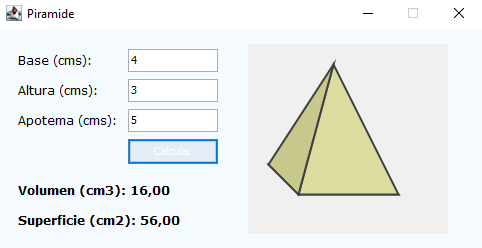
\includegraphics[width=\linewidth]{imagenes/8}
            \caption{Datos de la Pirámide.}
        \end{minipage}
    \end{figure}

    \item \textbf{Prevención de errores:} Igual que en el ejercicio anterior, controlamos que si pones letras en vez de números, el programa te avise.
    \begin{figure}[htbp]
        \centering
        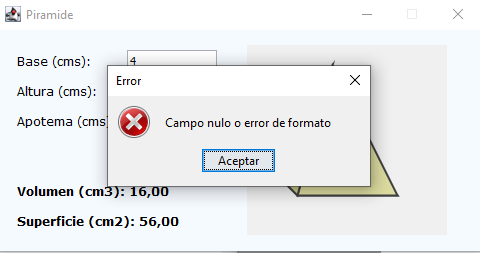
\includegraphics[width=0.45\textwidth]{imagenes/9}
        \caption{Aviso de error en el formato.}
    \end{figure}
\end{enumerate}

\subsection{Diagrama de Clases (UML)}
Se agregó información de las clases internas (\textit{PanelGrafico}) usadas para dibujar los sólidos mediante la librería Graphics2D.

\begin{figure}[htbp]
\begin{center}
\resizebox{\textwidth}{!}{%
\begin{tikzpicture}[
  font=\sffamily,
  inheritance/.style={draw=inheritColor, line width=1.2pt, -{Triangle[open, length=10pt, width=12pt]}},
  association/.style={draw=assocColor, line width=0.8pt, -{Latex[length=6pt, width=7pt]}},
  label/.style={font=\scriptsize\sffamily, fill=white, inner sep=2pt, rounded corners=2pt, text=assocColor},
  multiplicity/.style={font=\scriptsize\sffamily, fill=white, inner sep=1pt, text=assocColor}
]

\umlclass{Principal}{(0,1.5)}{3.0cm}{headerBlue}{Principal}{\strut}{+main(String[] args)\$}

\umlclass{VentanaPrincipal}{(0,-2.5)}{4.7cm}{headerBlue}{VentanaPrincipal}{%
-btnCilindro: JButton\\
-btnEsfera: JButton\\
-btnPiramide: JButton}{%
+VentanaPrincipal()\\
+actionPerformed(ActionEvent e)}

\umlclass{VentanaCilindro}{(-7.5,-9.0)}{4.8cm}{headerBlue}{VentanaCilindro}{%
-contenedor: Container\\
-radio: JLabel\\
-altura: JLabel\\
-volumen: JLabel\\
-superficie: JLabel\\
-campoRadio: JTextField\\
-campoAltura: JTextField\\
-calcular: JButton\\
-panelGrafico: PanelGrafico}{%
+VentanaCilindro()\\
+actionPerformed(ActionEvent evento)}

\umlclass{PanelCil}{(-7.5,-15.5)}{3.8cm}{headerBlue}{PanelGrafico}{}{+paintComponent(Graphics g)}
\draw[association] (VentanaCilindro.south) -- (PanelCil.north) node[label, midway, right] {Inner Class};


\umlclass{VentanaEsfera}{(0.0,-9.0)}{4.5cm}{headerBlue}{VentanaEsfera}{%
-contenedor: Container\\
-radio: JLabel\\
-volumen: JLabel\\
-superficie: JLabel\\
-campoRadio: JTextField\\
-calcular: JButton\\
-panelGrafico: PanelGrafico}{%
+VentanaEsfera()\\
+actionPerformed(ActionEvent evento)}

\umlclass{PanelEsf}{(0.0,-15.5)}{3.8cm}{headerBlue}{PanelGrafico}{}{+paintComponent(Graphics g)}
\draw[association] (VentanaEsfera.south) -- (PanelEsf.north) node[label, midway, right] {Inner Class};


\umlclass{VentanaPiramide}{(7.5,-9.0)}{4.8cm}{headerBlue}{VentanaPiramide}{%
-contenedor: Container\\
-base: JLabel\\
-altura: JLabel\\
-apotema: JLabel\\
-volumen: JLabel\\
-superficie: JLabel\\
-campoBase: JTextField\\
-campoAltura: JTextField\\
-campoApotema: JTextField\\
-calcular: JButton\\
-panelGrafico: PanelGrafico}{%
+VentanaPiramide()\\
+actionPerformed(ActionEvent evento)}

\umlclass{PanelPir}{(7.5,-15.5)}{3.8cm}{headerBlue}{PanelGrafico}{}{+paintComponent(Graphics g)}
\draw[association] (VentanaPiramide.south) -- (PanelPir.north) node[label, midway, right] {Inner Class};


\umlclass{Cilindro}{(-7.5,-21.5)}{4.0cm}{headerGreen}{Cilindro}{%
-radio: double\\
-altura: double}{%
+Cilindro(double r, double a)\\
+calcularVolumen(): double\\
+calcularSuperficie(): double}

\umlclass{Esfera}{(0.0,-21.5)}{3.8cm}{headerGreen}{Esfera}{%
-radio: double}{%
+Esfera(double r)\\
+calcularVolumen(): double\\
+calcularSuperficie(): double}

\umlclass{Piramide}{(7.5,-21.5)}{4.5cm}{headerGreen}{Piramide}{%
-base: double\\
-altura: double\\
-apotema: double}{%
+Piramide(double b, double h, double a)\\
+calcularVolumen(): double\\
+calcularSuperficie(): double}

\umlclass{FiguraGeometrica}{(0.0,-27.5)}{4.7cm}{headerGreen}{FiguraGeometrica}{%
-volumen: double\\
-superficie: double}{%
+setVolumen(double)\\
+setSuperficie(double)\\
+getVolumen(): double\\
+getSuperficie(): double}

\begin{scope}[on background layer]
  \node[
    draw=headerGreen!50,
    dashed,
    rounded corners=8pt,
    very thick,
    fill=headerGreen!5,
    inner xsep=15pt,
    inner ysep=15pt,
    fit=(Cilindro) (Esfera) (Piramide) (FiguraGeometrica)
  ] (namespace2) {};
  \node[
    anchor=south west,
    text=headerGreen,
    font=\bfseries\sffamily
  ] at (namespace2.north west) {Lógica de Negocio};
\end{scope}

\draw[association] (Principal.south) -- (VentanaPrincipal.north) node[label, midway, right] {Inicia};
\draw[association] (VentanaPrincipal.south) -- (VentanaEsfera.north);
\draw[association] (VentanaPrincipal.south) -| (VentanaCilindro.north);
\draw[association] (VentanaPrincipal.south) -| (VentanaPiramide.north);

\draw[association] (PanelCil.south) -- (Cilindro.north);
\draw[association] (PanelEsf.south) -- (Esfera.north);
\draw[association] (PanelPir.south) -- (Piramide.north);

\draw[inheritance] (Cilindro.south) -- ++(0,-1.5) -| (FiguraGeometrica.north);
\draw[inheritance] (Esfera.south) -- (FiguraGeometrica.north);
\draw[inheritance] (Piramide.south) -- ++(0,-1.5) -| (FiguraGeometrica.north);

\end{tikzpicture}%
}
\end{center}
\end{figure}

\section{Cómo probar el proyecto y Menú Principal}
Para que todo sea más fácil de revisar y no tener los archivos sueltos, creamos una ventana extra de \textbf{Menú Principal} (\textit{MenuActividad3}). Este menú agrupa todo y te deja saltar entre el sistema de Notas y el de las Figuras sin salir del programa.

\begin{figure}[htbp]
    \centering
    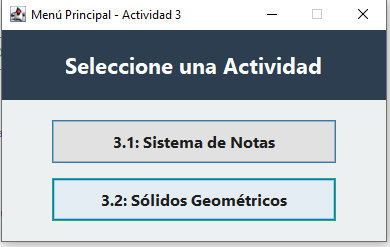
\includegraphics[width=0.45\textwidth]{imagenes/10}
    \caption{El menú que unifica toda la actividad 3.}
\end{figure}

Para correrlo, solo hay que abrir una consola en la carpeta raíz y ejecutar el archivo `.jar` que ya dejamos compilado, usando este comando:
\begin{verbatim}
java -jar Actividad_3_Menu.jar
\end{verbatim}

\subsection{Repositorio}
El proyecto está subido aquí: \url{https://github.com/cioranemil/poo-trabajo}

\end{document}
